% =====================================================================
% Age of Confidence: theory note (task A5 of the AoC plan), version 2
% Written for a broad audience: one running example, every equation
% introduced in words, every symbol defined after its equation.
% Format: IEEE conference, class IEEEtran V1.8b (the class of the
% official IEEE conference template, conference_101719.tex).
% Compile: pdflatex aoc_theory_note.tex (twice)
% All numbers come from the scripts in code/ (run code/a5_figures.py).
% =====================================================================
\documentclass[conference]{IEEEtran}
\IEEEoverridecommandlockouts
\usepackage{cite}
\usepackage{amsmath,amssymb,amsfonts}
\usepackage{graphicx}
\usepackage{textcomp}
\usepackage{xcolor}
\usepackage{booktabs}
\usepackage{array}
\usepackage{flushend}                   % balanced columns on the last page

\newcommand{\at}{\alpha^{\star}}             % target reliability
\newcommand{\Dl}{\Delta^{\star}}             % age limit
\newcommand{\aav}{\alpha_{\mathrm{avg}}}     % average reliability
\newcommand{\as}{\tilde{\alpha}}             % simple curve
\newcommand{\Dh}{\Delta_{1/2}}               % half-life
\newcommand{\Eq}[1]{Equation~(\ref{#1})}     % "Equation (n)", always spelled out
% compact list for the definitions that follow an equation
\newenvironment{where}{\begin{list}{\textbullet}{\setlength{\topsep}{2pt}\setlength{\partopsep}{0pt}%
\setlength{\itemsep}{0pt}\setlength{\parsep}{0pt}\setlength{\leftmargin}{1.5em}%
\setlength{\labelwidth}{0.6em}\setlength{\labelsep}{0.5em}}}{\end{list}}

\begin{document}

\title{Age of Confidence: How Often Must a Shared Object Be Updated?%
\thanks{Working note, version 3, October 25, 2026. The numerical values are
assumed. They are not yet fitted to real data.}}

% TODO (Godwin): check the author line and the affiliation, add co-authors.
\author{\IEEEauthorblockN{Godwin Koffi}
\IEEEauthorblockA{\textit{FEMTO-ST Institute, DISC Department} \\
\textit{Universit\'e de Technologie de Belfort-Montb\'eliard (UTBM)}\\
Belfort, France}}

\maketitle

\begin{abstract}
Connected vehicles share the objects they perceive in Collective Perception
Messages. When a receiver uses such an object, the object is already old.
Receivers today trust it fully up to a fixed age and then drop it. We propose
to compute the confidence that an aged object deserves. We define the
reliability of an object as the probability that it is still close to the
position that the receiver predicts, and we give a short formula for it. The
reliability stays close to one while the object is young and then falls. A
receiver that combines objects with belief functions can use it directly: the
older the object, the less it counts. We then compute the average reliability
when the object is updated at a given rate and some updates are lost. Finally,
we answer the reverse question: which update rate does an object need to reach
a target reliability? With assumed values and one update in ten lost, a moving
car needs one update every 0.6~s and a parked vehicle one every 9~s for the
same target. In the same conditions, regular updates need about half the rate
of updates sent at random times. A model in which the reliability falls from
the first instant asks for several times too many updates. A network
simulation of one link, with the real messages and radio, confirms the age
law and the formulas within 1.5\%.
\end{abstract}

\begin{IEEEkeywords}
collective perception, age of information, belief functions, discounting,
update rate, V2X
\end{IEEEkeywords}

% ---------------------------------------------------------------------
\section{Introduction}

A connected vehicle sees with more than its own sensors. Other vehicles and
roadside stations send it the objects they perceive, in Collective Perception
Messages (CPMs)~\cite{ts103324}. Fig.~\ref{fig:scenario} shows a typical case.
A pedestrian is about to cross the road. A parked truck hides the pedestrian
from the car on the left. A second car sees the pedestrian and shares the
position by radio. The first car now knows about a pedestrian that it cannot
see.

\begin{figure}[t]
\centering
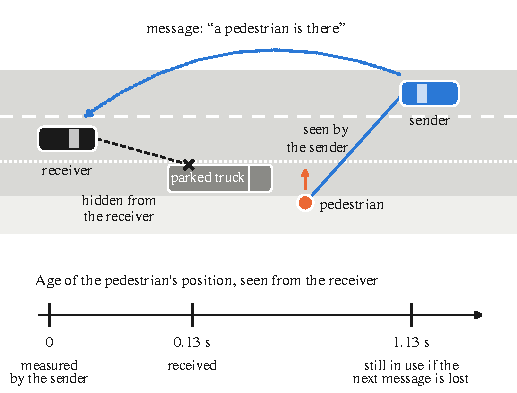
\includegraphics[width=\columnwidth]{figs/fig_scenario.pdf}
\caption{The situation studied in this paper. The sender sees a pedestrian
that the receiver cannot see, and shares it in a message. The position in the
message is already 0.13~s old when it arrives. If the next message, one second
later, is lost, the receiver still uses a position that is now 1.13~s old.}
\label{fig:scenario}
\end{figure}

But a shared object is never fresh. It was measured, processed, packed into a
message, sent, received and stored before the receiver uses it. If the next
message is lost, the receiver keeps the same object, and the object keeps
aging. Meanwhile the pedestrian walks on. The older the object, the less the
receiver knows where the pedestrian really is.

How much should the receiver trust an object that is 0.3~s old? And one that
is 2~s old? Current practice gives a yes-or-no answer. Evaluations count an
object as known only while its age is below 1~s~\cite{wolff2024}, and a
patented design discards a message when the age of its objects passes a fixed
limit~\cite{huang2024}. Studies of collective perception measure the age of
the objects inside the receiver, but they do not use this age when they
combine the objects~\cite{volk2021}. A fixed limit also ignores what the
object is. One second is long for a car that brakes. It is short for a parked
truck.

This paper asks two questions. What confidence does an object of a given age
deserve? And how often must the sender update the object to keep this
confidence above a target? Kaul \emph{et al.} asked how often a sender should
update a receiver so that the receiver holds fresh
information~\cite{kaul2012}. They measured freshness by the age. We ask the
same question for confidence. Unlike age, confidence depends on how the object
moves.

\begin{figure*}[t]
\centering
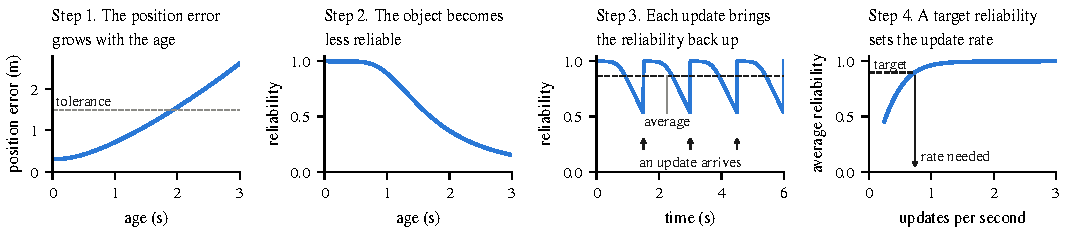
\includegraphics[width=\textwidth]{figs/fig_roadmap.pdf}
\caption{The four steps of the paper, drawn for a pedestrian. Sections
\ref{sec:step1} to \ref{sec:step4} take them one by one.}
\label{fig:roadmap}
\end{figure*}

We answer in four steps, shown in Fig.~\ref{fig:roadmap}. In Step~1, we
compute how the position error of an object grows with its age. In Step~2, we
turn this error into a \emph{reliability}: the probability that the object is
still close to the position that the receiver predicts. Belief function
theory, a framework to combine uncertain information, has an operation that
gives less weight to a source that is not fully reliable~\cite{shafer1976}.
The reliability is exactly the number that this operation needs. In Step~3, we compute the average
reliability when the sender updates the object at a given rate and some
updates are lost. In Step~4, we answer the reverse question and give the
update rate that a target reliability requires.

We keep the mathematics light. Each equation is introduced in words, and each
symbol is defined where it appears. One example runs through the whole paper:
the pedestrian of Fig.~\ref{fig:scenario}. Table~\ref{tab:notation} lists the
main symbols, and the longer derivations are in the appendices.

Three results stand out.
\begin{itemize}
\item The reliability does not fall steadily with age. It stays close to one
for a while, then falls. We call this first part the \emph{plateau}. A model
without a plateau asks for several times too many updates.
\item At the same rate, regular updates give more confidence than updates sent
at random times. For the same target they need about half the rate when few
updates are lost.
\item The required rate depends strongly on the object. For the same target, a
moving car needs one update every 0.6~s and a parked vehicle one every 9~s.
The current rules send the parked vehicle every second~\cite{ts103324}.
\end{itemize}

Our model is simple, and the numbers come from assumed values that are not yet
fitted to real data. We see the formulas, more than the numbers, as the
contribution. Section~\ref{sec:limits} states the limits of the model.

% ---------------------------------------------------------------------
\section{Related Work}\label{sec:related}

\emph{Age of information.} Kaul \emph{et al.}~\cite{kaul2012} define the age
of a status update as the time elapsed since the newest received update was
produced. Many results followed~\cite{yates2021}, also for vehicles that must
send less often because the radio channel is busy~\cite{turcanu2021,alsaqabi2026}.
In all these works the quantity of interest is the age itself. We turn the age
into a confidence that depends on the object.

\emph{Collective perception.} The European standard~\cite{ts103324} includes
an object in a CPM when its position, speed or direction has changed enough,
or after a maximum time. Such rules are compared by the load they put on the
channel and by the awareness they give~\cite{tr103562,thandavarayan2020}.
Awareness counts an object as known when its age is below a
limit~\cite{wolff2024}. None of these works derives a confidence from the
age.

\emph{Belief functions.} Belief function theory represents uncertain
statements and can also express ``I do not know''. Its discounting operation
weakens a statement by a reliability factor~\cite{shafer1976}, and later work
refines this operation~\cite{mercier2008}. These
works do not say where the factor comes from. We derive it from the age of the
object and from its motion.

% ---------------------------------------------------------------------
\section{Setting and Notation}\label{sec:model}

We consider one sender, one receiver and one pedestrian, as in
Fig.~\ref{fig:scenario}. The sender perceives the pedestrian and keeps an
estimate of the position and of the speed. From time to time, the sender puts
this estimate in a CPM. Seen from the receiver, this estimate is the
\emph{object}, and each transmission is an \emph{update} of the object. The
receiver keeps the last update that it received. Between two updates, it
assumes that the pedestrian keeps the same speed, and it moves the position
forward accordingly. We call the result the \emph{predicted position}.

\emph{Age.} Each update carries the time at which the object was measured. The
\emph{age} $\Delta$ of the object is the time elapsed since that measurement.
It is counted from the measurement, not from the reception. So the age is not
zero when an update arrives: the update needed some time to be processed and
transmitted. We call this time the \emph{delay} $d$. The evaluation
in~\cite{volk2021} puts it between 119 and 133 milliseconds, and we take
$d=0.13$~s.
After the arrival, the age grows by one second every second, until the next
update arrives and brings it back to $d$.

\emph{Updates and loss.} We study two ways of sending updates.
\emph{Regular updates} are sent every $T$ seconds, where $T$ is the
\emph{period}. \emph{Random updates} are sent at random instants, $\lambda$
times per second on average. An update is as likely at one moment as at any
other, whatever happened before, so the gaps between two updates are very
uneven. This case is called a Poisson process. It is the reference case in the
literature on the age of information~\cite{kaul2012}. In both cases we call $\lambda$ the \emph{update
rate}, in updates per second (Hz). For regular updates, $\lambda=1/T$. The
radio channel is not perfect. Each update is lost with probability $p$.
Losing one update does not make the next loss more or less likely.

\begin{table}[t]
\caption{Main symbols}
\label{tab:notation}
\centering
\begin{tabular}{@{}l@{\hspace{0.9em}}p{0.79\columnwidth}@{}}
\toprule
Symbol & Meaning \\
\midrule
$\Delta$ & age of the object: time since it was measured (s) \\
$d$ & delay: age of the object when an update arrives (0.13~s assumed; 1 to 92~ms in the simulation of Section~\ref{sec:check}) \\
$T$, $\lambda$ & period between two updates (s) and update rate
$\lambda=1/T$ (updates per second, Hz) \\
$p$ & probability that an update is lost \\
$\sigma_x$, $\sigma_v$ & typical error of the sender on the position (m) and
on the speed (m/s) of the object \\
$q$ & maneuver intensity: how strongly the object changes its speed at random
(m$^2$/s$^3$) \\
$\sigma(\Delta)$ & typical position error at age $\Delta$ (m) \\
$\varepsilon$ & tolerance: largest position error that the application
accepts (1.5~m) \\
$\alpha(\Delta)$ & reliability at age $\Delta$, between 0 and 1 \\
$\Dh$ & half-life: age at which the reliability is one half (s) \\
$L$, $\tau$ & plateau length and decay time of the simple curve $\as$ (s) \\
$\aav$ & average of the reliability over time \\
$\at$ & target reliability \\
$\Dl$ & age limit: age at which the reliability falls to $\at$ (s) \\
\bottomrule
\end{tabular}
\end{table}

% ---------------------------------------------------------------------
\section{Step 1: The Position Error Grows With the Age}\label{sec:step1}

The receiver predicts where the pedestrian is. How wrong can this prediction
be? Three errors combine.

\emph{The position error of the sender.} When the sender measured the
pedestrian, its estimate of the position was already off by a typical error
$\sigma_x$.

\emph{The speed error of the sender.} The estimate of the speed is off by a
typical error $\sigma_v$. A wrong speed moves the predicted position away from
the true one, a little more every second. After $\Delta$ seconds, the
resulting position error is $\Delta\,\sigma_v$.

\emph{The maneuvers of the object.} The pedestrian does not keep exactly the
same speed. The pedestrian speeds up, slows down or turns a little, and the
receiver cannot know it. We model these changes as small random pushes. Their
strength is a single number $q$, which we call the \emph{maneuver intensity}.
A calm object has a small $q$.

By ``typical error'' we mean a standard deviation: in one direction, about two
errors out of three are smaller than it. The three errors are independent.
Independent errors do not simply add, because they sometimes cancel each
other. It is their squares that add:
\begin{equation}\label{eq:sigma}
\sigma^2(\Delta)=\sigma_x^2+(\Delta\,\sigma_v)^2+\frac{q\,\Delta^3}{3},
\end{equation}
where
\begin{where}
\item $\sigma(\Delta)$ is the typical position error of the prediction at age
$\Delta$, in meters;
\item $\sigma_x$ is the typical position error of the sender at the
measurement time, in meters;
\item $\sigma_v$ is the typical speed error of the sender, in meters per
second;
\item $q$ is the maneuver intensity, in m$^2$/s$^3$;
\item $\Delta$ is the age, in seconds.
\end{where}
The last term needs a word. The maneuver intensity $q$ tells how fast the
speed drifts: after $\Delta$ seconds of random pushes, the speed has typically
changed by $\sqrt{q\Delta}$. With $q=0.5$, this is 0.7~m/s after one second.
Each change of speed then moves the position, and an early push has more time
to act than a late one. Adding up all the pushes over the age gives
$q\Delta^3/3$. This is the classical result for an object that moves at a
nearly constant speed~\cite{barshalom2001}. \Eq{eq:sigma} describes one
direction, for example along the road. We use the same value across the
road.\footnote{If the position
error and the speed error of the sender are linked, a term
$2\Delta\,\sigma_{xv}$ is added to \Eq{eq:sigma}, where $\sigma_{xv}$ measures
this link (their covariance). We take it equal to zero.}

\emph{Example.} For the pedestrian we take $\sigma_x=0.3$~m,
$\sigma_v=0.5$~m/s and $q=0.5$~m$^2$/s$^3$. Section~\ref{sec:objects} explains
these values. At the age of 1~s, \Eq{eq:sigma} gives
$\sigma^2=0.09+0.25+0.17=0.51$~m$^2$, so $\sigma=0.71$~m. At 2~s it gives
$\sigma^2=0.09+1.00+1.33=2.42$~m$^2$, so $\sigma=1.56$~m. The error does not
grow in a straight line. It is small at first and then grows faster and faster
(Fig.~\ref{fig:roadmap}, Step~1). At 1~s the largest part comes from the speed
error. At 2~s it comes from the maneuvers.

% ---------------------------------------------------------------------
\section{Step 2: From Position Error to Reliability}\label{sec:step2}

\subsection{Definition}

Is an error of 0.7~m a lot? It depends on what the receiver does with the
object. We therefore introduce a \emph{tolerance} $\varepsilon$: the largest
position error that the application accepts. We take $\varepsilon=1.5$~m,
about half the width of a lane. With this tolerance, an object is useful as
long as it tells which lane the pedestrian is in.

We define the \emph{reliability} of an object as the probability that the true
position is within the tolerance of the predicted position.
Fig.~\ref{fig:reliability} (top) shows the idea. Each dot is one position
where the pedestrian may really be, given what the receiver knows. The circle
has the radius $\varepsilon$ around the predicted position. The reliability is
the share of the dots inside the circle. When the object is fresh, all the
dots are inside. As the object ages, the cloud spreads and more dots fall
outside.

To compute this share, we assume that the error follows the bell-shaped
Gaussian law, with the typical size $\sigma(\Delta)$ in each of the two
directions. The share of the dots inside the circle is then
(Appendix~\ref{app:alpha})
\begin{equation}\label{eq:alpha}
\alpha(\Delta)=1-\exp\!\left(-\frac{\varepsilon^2}{2\,\sigma^2(\Delta)}\right),
\end{equation}
where
\begin{where}
\item $\alpha(\Delta)$ is the reliability at age $\Delta$, between 0 and 1;
\item $\varepsilon$ is the tolerance, in meters;
\item $\sigma(\Delta)$ is the typical position error given by \Eq{eq:sigma};
\item $\exp$ is the exponential function: $\exp(x)=e^x$, with $e\approx2.72$.
\end{where}

\Eq{eq:alpha} is easy to read. Only the ratio between the tolerance and the
typical error matters. When the error is small compared with the tolerance,
the exponential is almost zero and the reliability is almost one. When the
error equals the tolerance, the reliability is $1-e^{-1/2}=0.39$. This is less
than the two out of three quoted in Step~1, because the pedestrian can now be
off in two directions at once.

\emph{Example.} For the pedestrian at the age of 1~s, $\sigma=0.71$~m and
\Eq{eq:alpha} gives $\alpha=0.89$. Out of 100 possible positions, 89 are
within 1.5~m of the predicted one. At 2~s, $\sigma=1.56$~m and $\alpha=0.37$.

\begin{figure}[t]
\centering
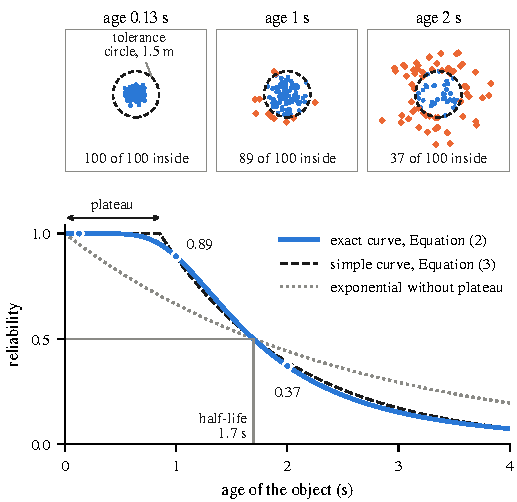
\includegraphics[width=\columnwidth]{figs/fig_reliability.pdf}
\caption{Reliability of the pedestrian. Top: 100 possible positions of the
pedestrian around the predicted position, at three ages. The reliability is
the share of the positions inside the tolerance circle. Bottom: the
reliability against the age. The three marked points are the three ages of the
top row. The dashed curve is the simple curve used in Step~3. An exponential
that falls from the first instant (dotted) misses the plateau.}
\label{fig:reliability}
\end{figure}

\subsection{Plateau and Half-Life}

Fig.~\ref{fig:reliability} (bottom) shows the reliability of the pedestrian
against the age (solid curve). Two features matter.

First, the curve has a plateau. It stays close to one as long as the error is
small compared with the tolerance. The reliability of the pedestrian is still 0.998
at the age of 0.5~s. Only then does it fall.

Second, we can sum up the speed of the fall by one number. We use the
\emph{half-life} $\Dh$: the age at which the reliability has fallen to one
half. For the pedestrian, $\Dh=1.7$~s. Appendix~\ref{app:ages} shows how to
compute it.

\subsection{A Simpler Curve for the Next Step}

In Step~3 we will average the reliability over time. \Eq{eq:alpha} is exact,
but its average cannot be written as a short formula. So we replace the exact
curve by a simpler one, made of two pieces. The first piece is flat. The
second piece is an exponential fall:
\begin{equation}\label{eq:plateau}
\as(\Delta)=
\begin{cases}
1, & \text{if } \Delta\le L,\\[2pt]
\exp\!\big(-(\Delta-L)/\tau\big), & \text{if } \Delta> L,
\end{cases}
\end{equation}
where
\begin{where}
\item $\as(\Delta)$ is the approximate reliability at age $\Delta$;
\item $L$ is the \emph{plateau length}, in seconds: up to this age, the object
is treated as fully reliable;
\item $\tau$ is the \emph{decay time}, in seconds: after the plateau, the
reliability is divided by 2.72 every $\tau$ seconds. A small $\tau$ means a
fast fall.
\end{where}

We choose $L$ and $\tau$ so that the simple curve crosses the exact curve at
the levels 0.9 and 0.5 (Appendix~\ref{app:ages}). For the pedestrian,
$L=0.85$~s and $\tau=1.22$~s. The dashed curve of Fig.~\ref{fig:reliability}
shows the result. The two curves never differ by more than 0.06, for all the
objects of Table~\ref{tab:params}.

Why not something even simpler? The simplest choice would be an exponential
that falls from the first instant, with no plateau. The dotted curve of
Fig.~\ref{fig:reliability} shows it for the same half-life. It misses the
plateau. For the pedestrian it is up to 0.24 below the exact curve before the
half-life, and up to 0.14 above it after. Step~4 will show that this error is
costly.

\subsection{Five Objects}\label{sec:objects}

Table~\ref{tab:params} lists the values that we use for five objects. For a
moving object, we assume that the sender knows the position within
$\sigma_x=0.3$~m and the speed within $\sigma_v=0.5$~m/s. To set the maneuver
intensity $q$, we use two numbers that are easier to picture: the typical
acceleration $\sigma_a$ of the object and the typical duration $\tau_m$ of one
of its maneuvers. Then $q=2\sigma_a^2\tau_m$. This relation matches our random
pushes to a classical maneuver model~\cite{singer1970}. Our model then
predicts a slightly larger error than the classical one, never a smaller one.
For the pedestrian, $\sigma_a=0.5$~m/s$^2$ and
$\tau_m=1$~s give $q=0.5$~m$^2$/s$^3$.

All these values are assumed. We chose them as plausible, and we did not
measure them. They must be fitted to recorded trajectories before the numbers
of this paper can be trusted. Even so, the table already shows one thing. The
half-life goes from 1~s for a moving car to 14~s for a parked vehicle. What an
object is doing matters more than what it is.

\begin{table}[t]
\caption{Assumed values for five objects and resulting constants
($\varepsilon=1.5$~m)}
\label{tab:params}
\centering
\begin{tabular}{@{}lcccccc@{}}
\toprule
Object & $\sigma_a$ & $\tau_m$ & $q$ & $\Dh$ & $L$ & $\tau$ \\
 & (m/s$^2$) & (s) & (m$^2$/s$^3$) & (s) & (s) & (s) \\
\midrule
Car, moving     & 1.0 & 2.0 & 4.00  & 0.99  & 0.54 & 0.64 \\
Truck, moving   & 0.6 & 2.0 & 1.44  & 1.32  & 0.70 & 0.89 \\
Bicycle         & 0.7 & 1.0 & 0.98  & 1.45  & 0.76 & 1.00 \\
Pedestrian      & 0.5 & 1.0 & 0.50  & 1.70  & 0.85 & 1.22 \\
Vehicle, parked & n.a. & n.a. & 0.001 & 13.88 & 5.79 & 11.67 \\
\bottomrule
\multicolumn{7}{@{}p{0.95\columnwidth}@{}}{\footnotesize Moving objects:
$\sigma_x=0.3$~m, $\sigma_v=0.5$~m/s. Parked vehicle: $\sigma_x=0.5$~m,
$\sigma_v=0.05$~m/s, $q$ set directly (n.a.: not applicable). $\sigma_a$:
typical acceleration. $\tau_m$: typical duration of a maneuver.}
\end{tabular}
\end{table}

\subsection{Using the Reliability in a Fusion}

The receiver combines the objects that it receives with what its own sensors
see. This step is called fusion. What should the fusion do with the
reliability? Belief function theory gives a direct answer~\cite{shafer1976}.
In this theory, a source shares one unit of belief between statements, and one
of the statements can be ``I do not know''. The shares are called
\emph{masses}. Suppose that the message of the sender says ``a pedestrian is
there'' with a mass of 0.9 and ``I do not know'' with a mass of 0.1.

Here the source is the aged object. Its message is true only if the pedestrian
is still where the receiver predicts, and the reliability $\alpha$ is the
probability of that. When a source is not fully reliable, the receiver weakens
its message. This operation is called \emph{discounting}~\cite{shafer1976}:
\begin{equation}\label{eq:discount}
\begin{aligned}
m^{\alpha}(B)&=\alpha\,m(B)\quad\text{for every statement } B\neq\Omega,\\
m^{\alpha}(\Omega)&=1-\alpha+\alpha\,m(\Omega),
\end{aligned}
\end{equation}
where
\begin{where}
\item $m(B)$ is the mass that the sender gives to the statement $B$;
\item $\Omega$ stands for ``I do not know''. Formally, it is the set of all
the possible answers;
\item $\alpha$ is the reliability of the source, here given by \Eq{eq:alpha};
\item $m^{\alpha}$ is the weakened message that the receiver uses.
\end{where}

\Eq{eq:discount} multiplies the mass of every statement by $\alpha$ and moves
the rest to ``I do not know''. Fig.~\ref{fig:discount} shows the effect on our
message. At the age of 1~s, the receiver keeps a mass of 0.80 for ``a
pedestrian is there''. At the half-life it keeps 0.45, and at 3~s only 0.14.
The object is never dropped all at once. It fades out.

A word on notation: many works call $1-\alpha$ the discount rate, and some
denote it by $\alpha$~\cite{shafer1976}. Here $\alpha$ is always a
reliability: 1 means full trust.

\begin{figure}[t]
\centering
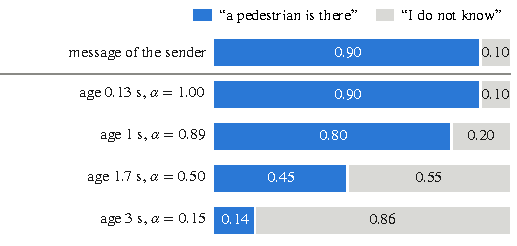
\includegraphics[width=\columnwidth]{figs/fig_discount.pdf}
\caption{What the receiver keeps of a message that says ``a pedestrian is
there'' with a mass of 0.9. The older the object, the lower its reliability
$\alpha$, and the more mass moves to ``I do not know''
(\Eq{eq:discount}).}
\label{fig:discount}
\end{figure}

% ---------------------------------------------------------------------
\section{Step 3: Average Reliability Under Repeated Updates}\label{sec:step3}

So far we looked at one update that grows old. In practice the sender sends
updates again and again. Fig.~\ref{fig:sawtooth} shows what happens at the
receiver. The age (top) grows, and falls back to the delay $d$ each time an
update arrives. It looks like the teeth of a saw. The reliability (bottom)
follows. It stays on the plateau, starts to fall, and comes back up when the
next update arrives. If an update is lost, the age keeps growing for one more
period, and the reliability falls much lower. The dashed lines mark a level of
0.9 that Step~4 will use as a target.

The reliability thus changes all the time. To sum it up by one number, we use
its average over time, $\aav$. It is the reliability that the receiver finds
on average when it looks at the object at an arbitrary moment.

\begin{figure}[t]
\centering
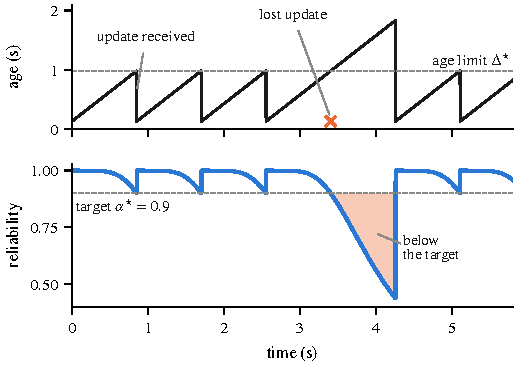
\includegraphics[width=\columnwidth]{figs/fig_sawtooth.pdf}
\caption{Age of the pedestrian at the receiver (top) and its reliability
(bottom), with one update every 0.85~s and one lost update. Each received
update brings the age back to the delay $d$. The dashed lines mark the target
used in Step~4: a reliability of 0.9, which the pedestrian reaches at the age
of 0.98~s. The reliability falls below this target only after the lost
update.}
\label{fig:sawtooth}
\end{figure}

\subsection{Regular Updates Without Loss}

We start with the simplest case: one update every $T$ seconds, and no loss.
Every period then looks the same, and we use the simple curve of
\Eq{eq:plateau}. At the start of a period, the object has the age $d$. It
stays on the plateau until its age reaches $L$, that is for $L-d$ seconds.
During this time its reliability is 1. During the rest of the period, that is
for $T-(L-d)$ seconds, the reliability falls. The average is the area under
the curve over one period, divided by the period:
\begin{equation}\label{eq:regular}
\aav=\frac{1}{T}\left[(L-d)+\tau\left(1-e^{-(T-(L-d))/\tau}\right)\right],
\end{equation}
where $T$ is the period, $L$ and $\tau$ are the plateau length and the decay
time of \Eq{eq:plateau}, and $d$ is the delay. In the brackets, the first term
$L-d$ is the time spent on the plateau, and the second term is the area under
the falling part of the curve. \Eq{eq:regular} holds when $T\ge L-d$. If $T$
is shorter, the next update arrives before the object leaves the plateau, and
$\aav=1$. Sending more often does not help.

\emph{Example.} For the pedestrian, $L-d=0.85-0.13=0.72$~s. With one update
per second, \Eq{eq:regular} gives $\aav=(0.72+0.25)/1=0.97$. With one update
every 2~s, it gives $\aav=(0.72+0.79)/2=0.76$.

\subsection{Lost Updates}

With loss, the periods are no longer alike. When an update is lost, the
receiver keeps the previous one. The age then reaches $d+2T$ before the next
update can arrive. If two updates in a row are lost, it reaches $d+3T$, and so
on. A run of $k$ lost updates has the probability $p^k$. The average takes all
these cases into account, each with its probability. The result is still a
formula, but a longer one: \Eq{eq:regularloss} in
Appendix~\ref{app:averages}.

\emph{Example.} For the pedestrian with one update per second, the average
reliability is 0.97 without loss. It is 0.92 when 10\% of the updates are
lost, and 0.81 when 30\% are lost.

\subsection{Random Updates}

For random updates, the average reliability has a short formula:
\Eq{eq:random} in Appendix~\ref{app:averages}. At the same rate and with the same loss, random updates always give a lower
average than regular updates. For the pedestrian with one update per second
and a loss of 10\%, the average is 0.75 against 0.92. Long gaps do the
damage, and random updates make them more likely. The reliability that is lost
during a long gap is not won back during the short ones, because the
reliability cannot go above one. Regular updates leave no long gaps.

\subsection{How Accurate Are the Formulas?}

The formulas of this section use the simple curve of \Eq{eq:plateau}. We
compared them with the average of the exact curve of \Eq{eq:alpha}, which we
computed point by point on a computer. Fig.~\ref{fig:expected} shows both for
the pedestrian when 30\% of the updates are lost. The lines are the formulas
and the markers are the exact values.

We also tested rates from 0.1 to 10 updates per second (0.02 to 1 for the
parked vehicle) and losses from 0 to 50\%. The formulas stay within 2.2\% of
the exact average for the moving objects, and within 5.1\% for the parked
vehicle. With the exponential that falls from the first instant, the error
reaches 19\% to 22\% for the moving objects. Finally, we simulated updates
that are sent and lost at random. The simulated average agrees with the
formulas within 0.002.

\begin{figure}[t]
\centering
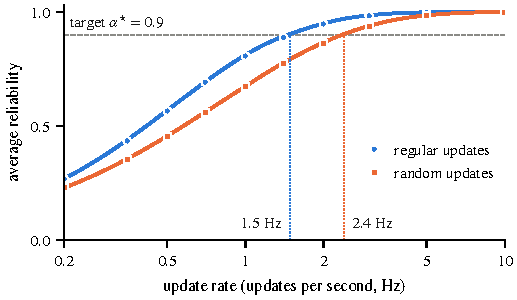
\includegraphics[width=\columnwidth]{figs/fig_expected.pdf}
\caption{Average reliability of the pedestrian against the update rate
(logarithmic scale), when 30\% of the updates are lost. Lines: formulas of
Step~3. Markers: exact curve, averaged on a computer. To reach an average of 0.9, regular updates need 1.5
updates per second and random updates 2.4.}
\label{fig:expected}
\end{figure}

% ---------------------------------------------------------------------
\section{Step 4: How Often Must an Object Be Updated?}\label{sec:step4}

We can now turn the question around. So far we chose an update rate and
computed the reliability. Now we choose a target reliability $\at$ and look
for the rate that reaches it. There are two reasonable ways to state the
target.

\subsection{A Target on the Average}

The first way is to require that the average reliability is at least the
target: $\aav\ge\at$. The average grows with the update rate
(Fig.~\ref{fig:expected}). So there is one smallest rate that reaches the
target, and we can read it on the figure. For the pedestrian with a loss of
30\%, the horizontal line at 0.9 crosses the two curves at 1.5 updates per
second for regular updates and at 2.4 for random updates. In practice a
computer finds this rate by trying values. Appendix~\ref{app:rates} gives
direct formulas for two cases.

\subsection{A Target on the Time Above a Level}

An average hides the bad moments. Take the pedestrian with regular updates, a
loss of 10\%, and the rate that gives an average of exactly 0.9. The
reliability is then below 0.9 for 30\% of the time. A stricter target limits
this time directly: the reliability must stay above $\at$ for most of the
time.

This target leads to a very simple rule. Let $\Dl$ be the age at which the
exact reliability of \Eq{eq:alpha} falls to the target $\at$. We call it the
\emph{age limit}. An update arrives with the age $d$. So the object stays
above the target for $\Dl-d$ seconds after each received update. The rule is
to send $n$ updates during this time:
\begin{equation}\label{eq:rule}
T=\frac{\Dl-d}{n},
\end{equation}
where $T$ is the period, $\Dl$ is the age limit, $d$ is the delay, and $n$ is
a whole number chosen by the designer: 1, 2, 3 and so on. With this period,
the reliability falls below the target only when $n$ updates in a row are
lost. This happens with the probability $p^n$. So the reliability is above the
target for a share $1-p^n$ of the time.

\emph{Example.} For the pedestrian and a target of 0.9, the age limit is
$\Dl=0.98$~s. With $n=1$, \Eq{eq:rule} gives $T=0.98-0.13=0.85$~s.
Fig.~\ref{fig:sawtooth} uses this period: the reliability touches the target
at the end of each period and goes below it only after the lost update. With a
loss of 10\%, the reliability is above the target for 90\% of the time with
$n=1$, and for 99\% of the time with $n=2$. Note that \Eq{eq:rule} uses the
exact curve. It does not need the simple curve.

\subsection{Required Rates}

Table~\ref{tab:rates} gives the update rates needed for a target of 0.9. All
the values are computed with the exact curve of \Eq{eq:alpha}.

First, regular updates need about half the rate of random updates when the
loss is 10\%. When the loss is 30\%, they need about 60\% of it
(Fig.~\ref{fig:expected}). Second,
\Eq{eq:rule} with $n=1$ keeps the reliability above 0.9 for 90\% of the time
when the loss is 10\%. It costs about 30\% more updates than the target on the
average. Third, the required rate differs by more than a factor of ten between
a moving car and a parked vehicle.

A model without a plateau would give a very different table. If the
reliability falls from the first instant, the object has already lost some
reliability when it arrives: after the delay of 0.13~s, the pedestrian is at
0.95 instead of 1. Little room is left above a target of 0.9. With a loss of
10\%, this model asks for about 5 times the rates of Table~\ref{tab:rates} for
the pedestrian, and for 16 to 18 times for the car.

\begin{table}[t]
\caption{Update rate (updates per second) needed for a target $\at=0.9$}
\label{tab:rates}
\centering
\begin{tabular}{@{}lccccc@{}}
\toprule
 & \multicolumn{4}{c}{Target on the average} & \Eq{eq:rule} \\
\cmidrule(lr){2-5}
 & \multicolumn{3}{c}{Regular updates} & Random & with $n=1$ \\
\multicolumn{1}{@{}r}{Updates lost:} & none & 10\% & 30\% & 10\% & any \\
\midrule
Car, moving     & 1.32 & 1.63 & 2.67 & 3.36 & 2.08 \\
Truck, moving   & 0.96 & 1.18 & 1.93 & 2.43 & 1.50 \\
Bicycle         & 0.86 & 1.07 & 1.74 & 2.19 & 1.36 \\
Pedestrian      & 0.74 & 0.91 & 1.49 & 1.87 & 1.17 \\
Vehicle, parked & 0.09 & 0.11 & 0.19 & 0.23 & 0.15 \\
\bottomrule
\multicolumn{6}{@{}p{0.95\columnwidth}@{}}{\footnotesize Exact curve of
\Eq{eq:alpha}, delay $d=0.13$~s. A rate of 0.11 means one update every 9~s.}
\end{tabular}
\end{table}

\subsection{Current Rules and Channel Limits}

How do these rates compare with what vehicles send today? The European
rules~\cite{ts103324} include a vehicle in a CPM when it has moved by 4~m, or
changed its speed by 0.5~m/s or its direction by 4 degrees, and at the latest
after 1~s. A car at 50~km/h moves 4~m in about 0.3~s, so it is sent about 3.3
times per second. Pedestrians and cyclists are included every 0.5~s.
Fig.~\ref{fig:rates} puts the two side by side. With our assumed values, the
current rules send every object more often than a target of 0.9 on the average
needs: about twice as often for the moving car, and nine times for the parked
vehicle. A stricter target changes the picture for fast objects. \Eq{eq:rule}
with $n=2$ asks for 4.2 updates per second for the car, which is more than the
rules send. These comparisons rest on assumed values, on one tolerance and on
one target. They only suggest where radio traffic can be saved, and parked
vehicles are the first candidates.

\begin{figure}[t]
\centering
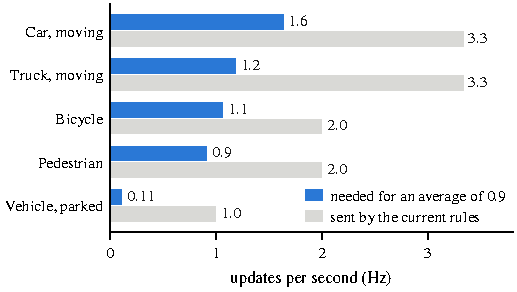
\includegraphics[width=\columnwidth]{figs/fig_rates.pdf}
\caption{Update rate needed for an average reliability of 0.9 (regular
updates, loss of 10\%), against the rate at which the current
rules~\cite{ts103324} send the object when the radio channel is free. Moving
vehicles are taken at 50~km/h. Assumed values, not fitted to data.}
\label{fig:rates}
\end{figure}

The radio channel also sets a limit. When the channel is busy, a mechanism
called decentralized congestion control makes every vehicle send less often.
In the example given by the standard~\cite{ts102687}, a vehicle may send 10
messages per second when the channel is busy less than 30\% of the time, and
only 1 message per second when it is busy more than 60\% of the time. With a
loss of 10\%, regular updates at 2 per second keep the average reliability
above 0.93 for every object of Table~\ref{tab:params}. At 1 per second, only
the pedestrian and the parked vehicle stay above 0.9, and the moving car falls
to 0.74. A target of 0.9 is therefore out of reach for fast objects when the
channel is very busy. The formulas of Step~3 then give the confidence that
remains.

% ---------------------------------------------------------------------
\section{Check in a Network Simulator}\label{sec:check}

\begin{figure*}[!t]
\centering
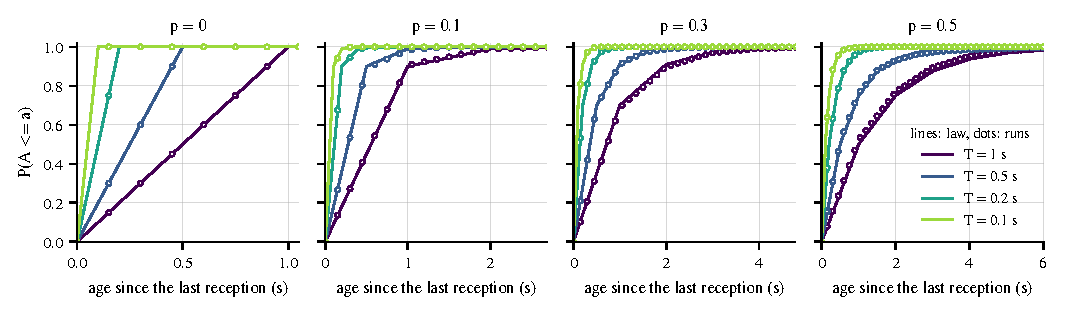
\includegraphics[width=\textwidth]{figs/fig_check_ages.pdf}
\caption{Share of time during which the age since the last reception is at
most $a$, in the 16 runs of the network simulation. Lines: the law of
Appendix~\ref{app:averages}. Dots: the runs. One panel per loss $p$, one
colour per period $T$.}
\label{fig:checkages}
\end{figure*}

\begin{figure*}[!t]
\centering
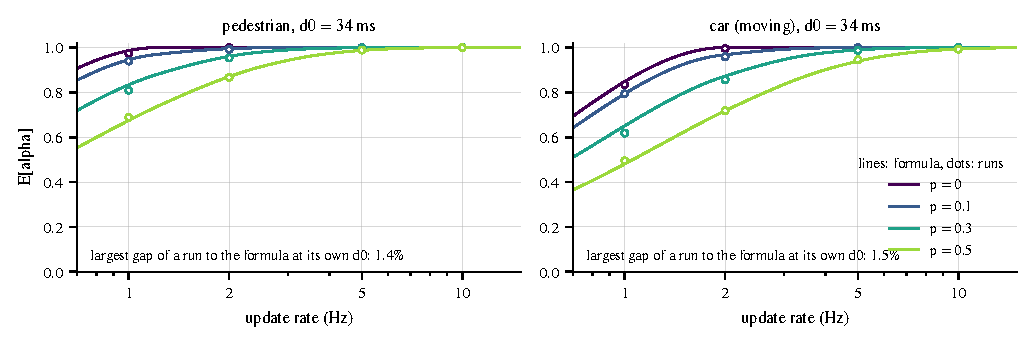
\includegraphics[width=\textwidth]{figs/fig_check_ealpha.pdf}
\caption{Average reliability against the update rate (logarithmic scale) in
the network simulation, for the pedestrian (left) and the moving car (right).
Lines: the formula of Step~3 with the simple curve, at the median delay of
the runs. Dots: the runs. The largest gap of a run to the formula is printed
in each panel.}
\label{fig:checkealpha}
\end{figure*}

The formulas of Step~3 rest on two things: the law of the age at the
receiver, and the average of the reliability over that law. We checked both
in a network simulation, with the real messages, the real radio and the
real timing of the sender.

\emph{Setup.} We used Artery~\cite{riebl2015}, which runs the ITS-G5 radio
and the Collective Perception Service of ETSI on top of OMNeT++ and
SUMO~\cite{lopez2018}. Three cars drive on a straight road at 10~m/s and
keep their distances: the receiver, then 180~m ahead the sender, then 40~m
ahead the object. The radars of the sender see the object; the radars of the
receiver, which reach 150~m, see nothing. So the receiver knows the object
only through the CPMs of the sender: one link, one object. The sender sends
a CPM with the object every $T$ seconds. The receiver drops each CPM with
probability $p$, independently of the others, which is the loss of our
model. We ran the 16 cases with $T$ in $\{1, 0.5, 0.2, 0.1\}$~s and $p$ in
$\{0, 0.1, 0.3, 0.5\}$, 330~s each, and we dropped the first 10~s. The CPMs
of the object about the sender give a second link of the same kind in every
run, so each run holds 334 to 6400 receptions. The period and the loss were
checked on the logs: the period is exact and the loss is within 0.02 of $p$.

\emph{Delay.} In the simulator, the radio takes less than one millisecond.
The delay $d$ is the time between the last radar step of the sender, at
10~Hz, and its CPM. It is between 1 and 92~ms depending on the run, with a
median of 34~ms over the runs, and it varies by up to 0.1~s inside a run. This
is below the 0.13~s of Table~\ref{tab:notation}, which includes the
processing of real equipment. In this section the formulas take the median
delay of each run.

\emph{The age law.} Over a run, the share of time during which the age since
the last reception is at most $a$ can be read exactly from the gaps between
receptions: it is the sum over the gaps $g$ of $\min(g,a)$, divided by the
length of the run. Fig.~\ref{fig:checkages} compares this share with the law
of Appendix~\ref{app:averages}, $P(A\le a)=1-p^k+(1-p)p^k r/T$ with
$a=kT+r$, for the 16 runs. The curves overlap. The largest distance between a
measured curve and the law is 0.04, and the mean age is within the noise of a
single run in every case: with $T=1$~s and $p=0.5$ a run holds only 334
receptions, and its mean age differs from $T/2+Tp/(1-p)$ by 7\%, where runs
drawn from the law itself differ by 6.5\% on average. Over the 16 runs the
gaps of the mean average to $-0.2\%$. At 10~Hz the distance of 0.04 comes from
the channel access: with three cars sending at 10~Hz, a CPM waits a few
milliseconds for the channel, which is a few percent of $T$.

\emph{The average reliability.} We then computed, on the same runs, the
average over time of the reliability $\alpha(\Delta)$ of \Eq{eq:alpha},
with the age of the object as the receiver saw it: the delay of each
reception plus the time since that reception. Fig.~\ref{fig:checkealpha}
shows it against the update rate for the pedestrian and the moving car, with
the formula of Step~3 (\Eq{eq:regularloss} with the simple curve) as lines.
For the five objects of Table~\ref{tab:params} and the 16 runs, the formula
is within 1.5\% of the simulation. The largest gaps are 1.4\% for the
pedestrian, 1.3\% for the bicycle, 1.5\% for the car, 1.1\% for the truck and
1.3\% for the parked vehicle, whose reliability at age zero is 0.989 and not
the 1 of the simple curve. The exact average of \Eq{eq:alpha} over the age
law is within 2.4\% of the simulation, within the noise of one run. The
exponential curve that falls from the first instant gives averages 3\% to
25\% too low on the moving objects, as in Section~\ref{sec:step3}.

\emph{What the check covers.} It covers the age law, the averaging and the
delay of a real sender, with the loss of the model. It does not test the
curve $\alpha(\Delta)$ itself: the cars drive straight, and the same curve is
used on both sides. Fitting $q$ on recorded trajectories remains the next
step. The loss is drawn at the receiver, so bursts of losses on a real
channel are not covered either (Section~\ref{sec:limits}).

% ---------------------------------------------------------------------
\section{Limits of the Model}\label{sec:limits}

\emph{Strong maneuvers.} Our random pushes are a fair model of small changes
of speed. A turn or a hard braking is different. The error then goes in one
direction and grows fast. With a constant braking of 2~m/s$^2$, the prediction
is off by 1.5~m after 1.2~s. A model made of random pushes does not cover this
case.

\emph{Loss.} We assumed that each loss is independent of the others. On a real
channel, losses come in bursts. We expect bursts to make long gaps more
likely, and so to lower the confidence.

\emph{Delay and values.} We took the delay as constant. A delay that varies
shortens the plateau by a random amount. In the simulation of
Section~\ref{sec:check} the delay varied by up to 0.1~s inside a run, and the
formulas with the median delay still held within 1.5\%. Finally, all the
numbers rest on Table~\ref{tab:params}. The formulas do not.

% ---------------------------------------------------------------------
\section{Conclusion}

We asked how much confidence an aged object deserves and how often it must be
updated. The answer fits in a few equations. \Eq{eq:sigma} gives the position
error of an object from its age, and \Eq{eq:alpha} turns this error into a
reliability that a fusion can use. \Eq{eq:regular} gives the average
reliability for a given update rate, and \Eq{eq:rule} the period that keeps
the reliability above a target.

The main lesson is that the right update rate depends on the object. A parked
vehicle and a moving car do not need the same number of updates. A network
simulation of one link, with the real messages and radio, confirms the age
law and the formulas within 1.5\%. The next steps are to fit the values to
recorded trajectories and to use the reliability in a fusion based on belief
functions.

% ---------------------------------------------------------------------
\appendices

\section{Where Equation (2) Comes From}\label{app:alpha}

Call $e_1$ and $e_2$ the errors of the predicted position along the road and
across it. We assume that they are independent and that each follows a
Gaussian law with a mean of zero and a standard deviation $\sigma$. The
distance between the predicted position and the true one is
$\rho=\sqrt{e_1^2+e_2^2}$. The probability that this distance is below the
tolerance, written $\Pr\{\rho\le\varepsilon\}$, is the integral of the Gaussian
law over the disc of radius $\varepsilon$. In polar coordinates,
\begin{equation}
\Pr\{\rho\le\varepsilon\}=\int_0^{\varepsilon}\frac{\rho}{\sigma^2}\,
e^{-\rho^2/(2\sigma^2)}\,d\rho=1-e^{-\varepsilon^2/(2\sigma^2)},
\end{equation}
which is \Eq{eq:alpha}. In practice the error is often larger in one direction
than in the other. Using the larger of the two values of $\sigma$ in
\Eq{eq:alpha} then gives a reliability that is never too
high~\cite{anderson1955}.

\section{Half-Life, Age Limit and Simple Curve}\label{app:ages}

At which age $\Delta_\ell$ does the reliability fall to a given level $\ell$?
Setting $\alpha(\Delta_\ell)=\ell$ in \Eq{eq:alpha} and using \Eq{eq:sigma}
gives
\begin{equation}\label{eq:level}
\frac{q}{3}\,\Delta_\ell^3+\sigma_v^2\,\Delta_\ell^2
=\frac{\varepsilon^2}{2\ln\!\big(1/(1-\ell)\big)}-\sigma_x^2 ,
\end{equation}
where $\ln$ is the natural logarithm. The left side grows with
$\Delta_\ell$, so \Eq{eq:level} has one solution when its right side is
positive. A computer finds it in a few steps. The level $\ell=1/2$ gives the
half-life $\Dh$. It exists when $\sigma_x<0.85\,\varepsilon$. The level
$\ell=\at$ gives the age limit $\Dl$ of Step~4.

The simple curve of \Eq{eq:plateau} crosses the exact curve at the levels 0.9
and 0.5. Call $\Delta_{0.9}$ and $\Delta_{0.5}$ the two ages given by
\Eq{eq:level}. Then
\begin{equation}
\tau=\frac{\Delta_{0.5}-\Delta_{0.9}}{\ln 2-\ln(10/9)},\qquad
L=\Delta_{0.9}-\tau\ln(10/9).
\end{equation}

\section{Average Reliability With Loss}\label{app:averages}

\emph{Regular updates.} Look at the receiver at an arbitrary moment. The last
sending instant was between 0 and $T$ seconds ago, and all the values in
between are equally likely. The update sent at that instant was received with
the probability $1-p$. If it was lost, the last received update is one period
older, and so on. So the time since the last received update lies between $kT$
and $(k+1)T$ with the probability $(1-p)\,p^k$, for $k=0,1,2$ and so on. The
age of the object is this time plus the delay $d$.

Now write $L-d=jT+r$, where $j$ is a whole number and $0\le r<T$. In words,
$j$ full periods fit in the time that the object spends on the plateau, and
$r$ is what remains. Averaging the simple curve of \Eq{eq:plateau} over all
the cases gives
\begin{multline}\label{eq:regularloss}
\aav=1-p^{j}+(1-p)\,p^{j}\Bigg[\frac{r}{T}\\
+\frac{\tau}{T}\left(1-\frac{(1-p)\,e^{-(T-r)/\tau}}
{1-p\,e^{-T/\tau}}\right)\Bigg].
\end{multline}
The term $1-p^{j}$ is the probability that fewer than $j$ updates in a row
were lost. The object is then still on the plateau. Without loss ($p=0$) and
with $T\ge L-d$ ($j=0$), \Eq{eq:regularloss} becomes \Eq{eq:regular}.

\emph{Random updates.} The received updates arrive at random instants, $\mu$
times per second on average, with $\mu=(1-p)\lambda$. The time since the last
received update is then longer than $t$ seconds with the probability
$e^{-\mu t}$. Averaging the simple curve gives
\begin{equation}\label{eq:random}
\aav=1-\frac{e^{-\mu(L-d)}}{1+\mu\,\tau}.
\end{equation}
Both formulas assume $L\ge d$, which holds for all the objects of
Table~\ref{tab:params}.

\section{Direct Formulas for the Required Rate}\label{app:rates}

\Eq{eq:random} can be solved for the rate. Write $u=(L-d)/\tau$. The smallest
rate of random updates that reaches the target $\at$ on the average is
\begin{equation}\label{eq:lmin}
\lambda_{\min}=\frac{1}{(1-p)\,\tau}\left[\frac{1}{u}\,
W\!\left(\frac{u\,e^{u}}{1-\at}\right)-1\right],
\end{equation}
% column break that balances the last page; remove it if the text changes
\newpage
\noindent where $W$ is the Lambert function~\cite{corless1996}: $W(x)$ is the number $w$
such that $w\,e^{w}=x$. Numerical libraries provide it, and we use its main
branch, the one that they return by default. For regular updates without
loss, \Eq{eq:regular} gives the longest period that reaches the
target:
\begin{equation}\label{eq:tmax}
T_{\max}=(L-d)+\frac{c}{\at}+\tau\,
W\!\left(-\frac{1}{\at}\,e^{-c/(\at\,\tau)}\right),
\end{equation}
with $c=(L-d)(1-\at)+\tau$. With loss, a computer solves
\Eq{eq:regularloss} by trying values: the average falls when the period grows,
so a search by successive halving finds the longest period. \Eq{eq:lmin} and \Eq{eq:tmax}
reproduce the values of Table~\ref{tab:rates} within 2\% for the moving
objects.

% ---------------------------------------------------------------------
\begin{thebibliography}{00}

\bibitem{ts103324} \emph{Intelligent Transport Systems (ITS); Vehicular
Communications; Basic Set of Applications; Collective Perception Service;
Release 2}, ETSI TS 103 324 V2.1.1, Jun. 2023.

\bibitem{wolff2024} V. A. Wolff, E. Xhoxhi, and F. Tautz, ``An application
layer multi-hop collective perception service for vehicular adhoc networks,''
arXiv:2404.07761, Apr. 2024.

\bibitem{huang2024} Y.-K. Huang and K.-P. Chang, ``Device and vehicle for V2X
system,'' U.S. Patent 12\,128\,926 B2, Oct. 29, 2024.

\bibitem{volk2021} G. Volk \emph{et al.}, ``Towards realistic evaluation of
collective perception for connected and automated driving,'' in \emph{Proc.
IEEE Int. Intell. Transp. Syst. Conf. (ITSC)}, 2021, pp. 1049--1056.

\bibitem{kaul2012} S. Kaul, R. Yates, and M. Gruteser, ``Real-time status: How
often should one update?'' in \emph{Proc. IEEE INFOCOM}, 2012,
pp. 2731--2735.

\bibitem{shafer1976} G. Shafer, \emph{A Mathematical Theory of Evidence}.
Princeton, NJ, USA: Princeton Univ. Press, 1976.

\bibitem{yates2021} R. D. Yates, Y. Sun, D. R. Brown, S. K. Kaul, E. Modiano,
and S. Ulukus, ``Age of information: An introduction and survey,'' \emph{IEEE
J. Sel. Areas Commun.}, vol. 39, no. 5, pp. 1183--1210, May 2021.

\bibitem{turcanu2021} I. Turcanu, A. Baiocchi, N. Lyamin, and A. Vinel, ``An
age-of-information perspective on decentralized congestion control in
vehicular networks,'' in \emph{Proc. Mediterranean Commun. Comput. Netw. Conf.
(MedComNet)}, 2021.

\bibitem{alsaqabi2026} Y. AlSaqabi, ``Age of information under DCC rate
constraints for V2I broadcast along urban corridors,'' arXiv:2606.29611,
Jun. 2026.

\bibitem{tr103562} \emph{Intelligent Transport Systems (ITS); Vehicular
Communications; Basic Set of Applications; Analysis of the Collective
Perception Service (CPS); Release 2}, ETSI TR 103 562 V2.1.1, Dec. 2019.

\bibitem{thandavarayan2020} G. Thandavarayan, M. Sepulcre, and J. Gozalvez,
``Generation of cooperative perception messages for connected and automated
vehicles,'' \emph{IEEE Trans. Veh. Technol.}, vol. 69, no. 12, Dec. 2020,
doi: 10.1109/TVT.2020.3036165.

\bibitem{mercier2008} D. Mercier, B. Quost, and T. Den{\oe}ux, ``Refined
modeling of sensor reliability in the belief function framework using
contextual discounting,'' \emph{Inf. Fusion}, vol. 9, no. 2, pp. 246--258,
2008.

\bibitem{barshalom2001} Y. Bar-Shalom, X. R. Li, and T. Kirubarajan,
\emph{Estimation with Applications to Tracking and Navigation}. New York, NY,
USA: Wiley, 2001.

\bibitem{singer1970} R. A. Singer, ``Estimating optimal tracking filter
performance for manned maneuvering targets,'' \emph{IEEE Trans. Aerosp.
Electron. Syst.}, vol. AES-6, no. 4, pp. 473--483, Jul. 1970.

\bibitem{anderson1955} T. W. Anderson, ``The integral of a symmetric unimodal
function over a symmetric convex set and some probability inequalities,''
\emph{Proc. Amer. Math. Soc.}, vol. 6, pp. 170--176, 1955.

\bibitem{corless1996} R. M. Corless, G. H. Gonnet, D. E. G. Hare,
D. J. Jeffrey, and D. E. Knuth, ``On the Lambert W function,'' \emph{Adv.
Comput. Math.}, vol. 5, pp. 329--359, 1996.

\bibitem{riebl2015} R. Riebl, H.-J. G\"unther, C. Facchi, and L. Wolf,
``Artery: Extending Veins for VANET applications,'' in \emph{Proc. Int. Conf.
Models Technol. Intell. Transp. Syst. (MT-ITS)}, 2015, pp. 450--456.

\bibitem{lopez2018} P. A. Lopez \emph{et al.}, ``Microscopic traffic
simulation using SUMO,'' in \emph{Proc. IEEE Int. Intell. Transp. Syst. Conf.
(ITSC)}, 2018, pp. 2575--2582.

\bibitem{ts102687} \emph{Intelligent Transport Systems (ITS); Decentralized
Congestion Control Mechanisms for Intelligent Transport Systems Operating in
the 5 GHz Range; Access Layer Part}, ETSI TS 102 687 V1.2.1, Apr. 2018.

\end{thebibliography}

\end{document}
